\documentclass[10pt,preprint]{sigplanconf}

% The following \documentclass options may be useful:

% preprint      Remove this option only once the paper is in final form.
% 10pt          To set in 10-point type instead of 9-point.
% 11pt          To set in 11-point type instead of 9-point.
% authoryear    To obtain author/year citation style instead of numeric.

\usepackage{graphicx}

\begin{document}

\newcommand{\charcoal}{Charcoal}

\special{papersize=8.5in,11in}
\setlength{\pdfpageheight}{\paperheight}
\setlength{\pdfpagewidth}{\paperwidth}

\conferenceinfo{CONF 'yy}{Month d--d, 20yy, City, ST, Country}
\copyrightyear{2014}
\copyrightdata{978-1-nnnn-nnnn-n/yy/mm}
\doi{nnnnnnn.nnnnnnn}

\titlebanner{Preprint.  Please do not redistribute}        % These are ignored unless
\preprintfooter{Preprint.  Please do not redistribute}   % 'preprint' option specified.

\title{Pseudo-Preemptive Threads: A New Multitasking Primitive for Reliable, Composable and Maintainable Software}
\subtitle{Why Events, Threads and Coroutines are All Bad Ideas\footnotemark}

\authorinfo{Benjamin Ylvisaker}
           {Affiliation1}
           {Email1}
\authorinfo{Name2\and Name3}
           {Affiliation2/3}
           {Email2/3}

\maketitle

\begin{abstract}
This is the text of the abstract.
\end{abstract}

\category{CR-number}{subcategory}{third-level}

% general terms are not compulsory anymore,
% you may leave them out
\terms
term1, term2

\keywords
keyword1, keyword2

\footnotetext{This tongue-in-cheek subtitle is a reference to Ousterhout \cite{Ousterhout1996} and von Behren, et al. \cite{Behren2003a}}

\section{Introduction}

It is hard to write multitasking software that is reliable, composable and maintainable.
The most popular abstractions for building such software (events, threads, coroutines) all have significant weaknesses.

This paper describes a new abstraction called \emph{pseudo-preemptive threads} (or \emph{activities}) that promises to make writing multitasking software easier.
To validate the ideas proposed in this paper we implemented activities in a dialect of C called \charcoal{}.
We wrote several microbenchmarks to explore the performance implications of activities.
% We also tweaked two real-world multithreaded C programs to use activities instead of threads to explore the software engineering implications.

This paper starts with brief a description and critique of the dominant multitasking abstractions.

Next we describe activities and provide abstract arguments for why activities do not suffer from the reliability, composability and maintainability weakness of other abstractions.

Next the paper describes the high points of the \charcoal{} implementation.
All the code for the implementation and tests described in this paper is available in a public repository on GitHub.

Finally, we report on the results of our microbenchmarks and real-world application implementations.

\subsection{Contributions}

This paper has two primary contributions:

\begin{itemize}
\item The definition of \emph{pseudo-preemptive threads} (a.k.a. \emph{activities}).
The most concise version is that they are similar to cooperative threads, with the addition of automatic yield insertion and a scoped no-yield primitive.
\item A new call frame allocation strategy for multithreaded programs called \emph{hot stacking}.
With this strategy long-lived call frames are individually heap allocated and most short-lived frames are allocated in a single shared contiguous memory area.
\end{itemize}

\section{Established Multitasking Abstractions}

The three most widely used multitasking frameworks are events, threads and coroutines.
Each suffers from serious software engineering problems that we categorize into reliability, composability and/or maintainability.
In this section we describe these problems; in later sections we argue that activities completely avoid or substantially mitigate all of them.

\subsection{Events}

Events are the most popular abstraction for relatively simple multitasking patterns; many GUI and network programming frameworks use events for things like mouse clicks, keyboard presses and receiving network messages.
Until recently this was the only available multitasking abstraction in some popular ecosystems (e.g. browser JavaScript).

When an event dispatcher calls a handler/listener procedure, that call must return before another event can be handled.
This makes avoiding many kinds of concurrency bugs easy.
However, it comes at a high cost in maintainability and reliability for complex applications.

Potentially long-running (or blocking) tasks must be manually broken up into smaller handler procedures by application programmers.
This leads to a style of programming referred to as \emph{stack ripping}\cite{Adya2002}, or more colloquially \emph{callback hell}.
Callback hell can make it hard to decipher the logical flow of a task, because it is split among  multiple callback procedures.
This is bad for reliability, because it is easy to make a mistake in the lifetime of some piece of data (compared with, for example, threads) \cite{Behren2003a}.
Callback hell is even worse for maintainability, because choices about how to break an application up into handlers can be hard to reconstruct down the road.

\subsection{Threads (Preemptive)}

Events are at the safest and least flexible end of the multitasking abstraction spectrum and threads occupy the opposite extreme.
(In this paper \emph{thread} means \emph{preemptive thread}.)

The primary strength of threads is that they can wait/block indefinitely and/or run for a very long time without preventing other threads from making progress.
This makes it possible to write multitasking software in a natural single-task style (i.e. threads completely avoid callback hell).

The primary weakness of threads is that it is extremely hard to avoid and remove concurrency bugs like data races, deadlocks, atomicity violations and livelocks.
In the last decade a significant amount of research effort has been devoted to making it easier to write reliable multithreaded applications, because of the emergence of mainstream multiprocessor computers.
While this body of work is quite impressive, most mainstream application programmers still view threads as too dangerous for multitasking programming (correctly in the current authors' opinion).

Applications that use threads and conventional concurrency control mechanisms also suffer from serious composability issues \cite{Harris2005, Grossman2007}.
The very brief summary of the arguments from the cited papers is that when using mutexes, semaphores and their cousins, application programmers must design and (somehow) enforce subtle global concurrency control properties.
Using transactions instead of conventional concurrency control mechanisms promises to make threads much safer and more composable.
Unfortunately, current implementations of transactional concurrency control systems have problems that have prevented widespread addoption so far.

Among the multitasking abstractions discussed in this paper, threads are unique in that they naturally allow the parallel execution of tasks.
From the perspective of multitasking, parallelism is mostly irrelevant; multitasking abstractions like events and coroutines can be used in tandem with parallelism abstractions like threads and processes.
Nevertheless, in the discussion section at the end of this paper we speculate on the feasibility of running activities in parallel.

\subsection{Coroutines}

Coroutines have an interesting history.
According to Knuth, the term was coined by Melvin Conway in 1958, but coroutines remained on the margins of mainstream software practice until quite recently, a gap of more than 5 decades.
A few examples of recent implementations: the async/await framework (coroutines by a different name) was added to C\# in version 5, which was released in 2012; \texttt{function*} (coroutines by a different name) was added to the 2015 revision of ECMAScript; D4134 is a proposal to add coroutines to C++17.

Our interpretation of this interesting history is that (1) coroutines are far from perfect as a multitasking primitive (otherwise they would have been widely adopted much sooner), and (2) mainstream applications have gotten more sophisticated in their use of multitasking, making life in callback hell ever more painful.
Coroutines have been adopted as the least bad alternative to events.

Using the coroutine abstraction requires application programmers to partition procedures into normal procedures (functions, methods, subroutines, whatever) and coroutines.
In most implementations the procedure calling syntax is overloaded; what appears to be a call to coroutine is actually a concurrent task spawn.
Within the body of a coroutine definition, a \emph{yield} (or \emph{await}) primitive can be used to permit switching execution flow to a different task (i.e. coroutine).
Invoking yield in a normal procedure (a non-coroutine) is not permitted.

Relative to event loops, coroutines provide greater flexibility, because multiple tasks can be in progress at the same time.
Coroutines are much more resistant to concurrency bugs than threads, because only one coroutine can be active at a time, and the application explicitly states when switching between tasks is permitted.

The primary weakness of coroutines is a subtle but nasty tension with conventional procedural abstraction.
It is common for application programmers to want to yield in a \emph{procedure} called by a coroutine, but this is not possible.
This can be quite inconvenient on its own, and it makes refactoring strategies like procedure extraction trickier to apply.
Another consequence of this issue is that coroutines tend to be viral; if a programmer decides to convert a procedure to a coroutine (for example because it needs to wait for the arrival of a network message), it tends to be the case that any callers of that procedure need to be converted to coroutines as well.

Similarly, higher-order function patterns get more complicated as well.
There are now two distinct types of procedure-like-things [clarify/expand].

These software engineering awkwardnesses have not prevented the adoption of coroutines, but they are annoying.
Activities solve these problems!

\subsection{Cooperative Threads}

Cooperative threads can be seen as a compromise between coroutines and threads.
Like coroutines, cooperative threads must invoke a yield primitive to switch from one task to another.
Like threads, cooperative threads do not have a separate kind of procedure (i.e. coroutine/async) and yield can be invoked anywhere (i.e. not restricted to coroutine bodies).

Cooperative threads have a tension with procedural abstraction that is complementary to the tension in coroutine abstractions.
The atomicity properties of a particular procedure depend on whether or not any of the procedures it calls will invoke yield.
This can be annoying when initially writing code, and it is especially problematic during maintenance.
If yield is added to a procedure that did not previously have it, there is the possibility that any caller of that procedure will have its atomicity properties violated.
This is extra nasty when indirect calls are considered, because it is not possible in general to identify all call sites to a particular procedure.

A quick note on terminology: It is fairly common to see the term \emph{coroutine} applied to what we call \emph{cooperative threads}.
In the context of such usage, what we call coroutines are often called \emph{stackless coroutines}.
Naturally, we prefer the terms as defined in this paper.

\subsection{Others}

There are other approaches to multitasking that we briefly mention here only to argue that they are not directly relevant to the main points of this paper.

Isolated processes can be used for multitasking, but are far too heavy for the kinds of applications we are focused on (like GUI events and asynchronous network downloads).

Functional reactive programming (FRP) is an entirely different approach to multitasking.
It is interesting, but still at an early enough stage of research that it is not clear whether it can be integrated with mainstream programming practice.

\section{Pseudo-Preemptive Threads}

Before defining pseudo-preemptive threads, we start with an example stolen from \cite{Krohn2007}.
This example concurrently fetches DNS information using the standard \texttt{getaddrinfo} procedure.

\hspace{-0.5cm}
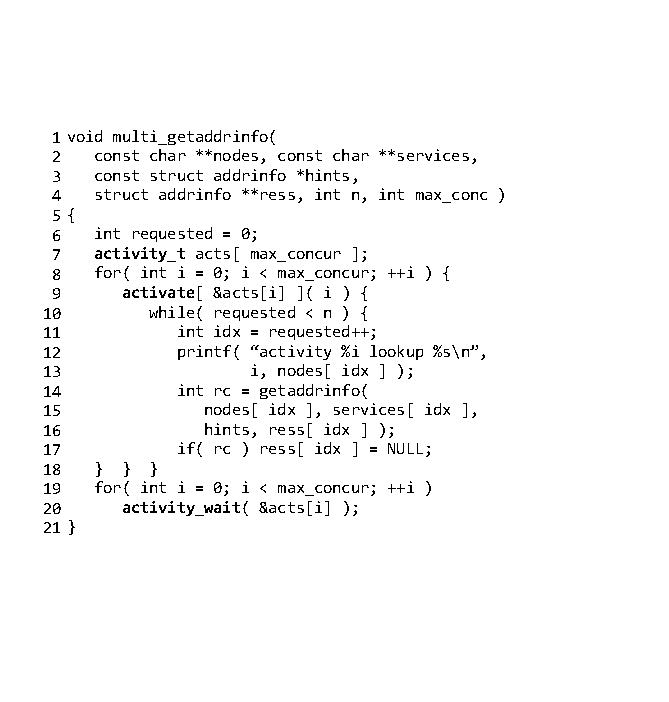
\includegraphics{multi_getaddrinfo}

There are things worth noting about this code.
The central syntactic addition is the \emph{activate} statement (line 10).
The body of an activate statement executes concurrently (but not in parallel) with whatever comes after the statement (i.e. its continuation).
The program can only switch between activities on a yield execution, but there are many implicit yields.
Any blocking or potentially long-running system call is rewritten to start, then yield.
Also every loop has an implicit (in the source code) yield at the end of every iteration.

These automatically-inserted yields make activities behave more like threads than events or coroutines from an application programmer's perspective.
However, there is a big difference between activities and threads.
Notice that multiple activities read and write the (shared) local variable \texttt{requested}.
If these were threads, this would cause a data race, which at best leads to unpredictable results and at worst makes the whole program undefined.
With activities this is not a problem at all; the system (compiler, processors, etc.) is not permitted to move memory operations across yields, which dramatically simplifies the concurrent memory model problem.

The activate statement takes as a parameter a pointer to application-allocated memory for storing necessary metadata about the new activity.
In the above example the memory for storing activity information is allocated locally.
Because of this the example procedure must wait for all the activities to finish.
(Returning before they finish would cause the runtime system to access deallocated memory).
It would be possible to change the interface so that the caller passes in the backing memory.
In that case, the procedure could return while the activities were still fetching DNS information, allowing the application to go on with other work.

Note that as compact as this example is, it incorporates a slightly fancy feature of limiting the number of concurrent network connections to an application-specified number.

The parentheses after the activate keyword are for controlling whether local variables are access by-value or by-reference.
The default is by-reference, which is how all the variables are used in this example.
In some cases it is more convenient to capture the value of a local variable at activation time.
This can be done by simply listing the variable inside the parentheses.
Making a local variable by-value effectively makes two copies of it that can be updated independently.

\subsection{Don't know}

Additionally, like all properly implemented cooperative threads, activities cannot suffer from data races

\cite{Boehm2011}

\subsection{Activate}

The activate statement creates a new activity, which runs concurrently with the activity that spawned it.
The runtime system is responsible for scheduling activities.
Context switching is only possible when an activity executes a yield primitive.
The semantics of a program with activities can be seen as batches of actions separated by yield invocations.
Batches from different activities are interleaved to execute a complete program.
Actions are not permitted to cross yield boundaries.
In other words, yields define the minimum granularity of interleaving.
In this way activities are identical to conventional cooperative threads.

\subsection{Yield Insertion}

What distinguishes activities from cooperative threads is yield insertion.
Informally, to support activities properly a language definition must ensure that a program cannot block or run indefinitely without executing a yield action.
This is achieved by automatically inserting yields in certain places before a program is compiled or interpreted.



Part of the definition of activities is that by default yields should happen ``frequently''.
But what does this mean precisely?
The answer depends on the details of the rest of the programming language definition.
However we can state two design rules that apply to any language.
These rules are in strong tension with each other:

\begin{enumerate}
\item It should \textbf{not} be possible for an activity to run indefinitely without executing a yield.
\item Yields should happen as infrequently as possible.
\end{enumerate}

One clear consequence of these rules is that anything that could cause an activity to pause indefinitely (e.g. a syscall) by default must be modified to allow other activities to run while the paused activity waits.
More challenging, loops must be interrupted.

\subsection{No-Yield}

If there was no way to limit yielding, activities would suffer from many of the same concurrency bug challenges as threads.
To combat this we add no-yield.
Any statement, expression or procedure declaration can be ``wrapped'' with no-yield.
In the dynamic scope of a no-yield block (statement, expression, procedure), the current activity cannot be interrupted.
This is a simple and powerful tool for enforcing atomicity.
We expect that most of the uses of locks in current multithreading practice can be directly replaced by the simpler and safer no-yield.

Because activities are like threads in that tasks can be written in a natural (not callback hell) style, activities do not suffer from the maintenance problems of events.
Because the primary concurrency control mechanism (no-yield) enforces a simple global property, activities do not suffer from the composability problems of threads.
Because the concurrency control is generally simple, activities do not suffer from the reliability problems of threads.
To be fair, applications written with activities will surely have concurrency bugs; it seems impossible to write multitasking software with zero exposure to concurrency bugs.
However, ...

With the addition of no-yield, activities can be seen as quite similar to coroutines with a complementary default.
Normal procedures in an activity framework are like coroutines and normal procedures in a coroutine framework are like no-yield procedures in an activity framework.
As similar as this argument makes coroutines and activities seem, we believe the differences are still significant.
For example, in an activities framework, all procedures are part of the same type; normal procedures and no-yield procedures are not distinguished at the type level.

\subsubsection{Recursive Procedure Calls}

The current design of \charcoal{} does not follow rule \#1 perfectly.
Function calls and returns do not implicitly yield, which means that recursion can be used to make an activity run indefinitely without yielding.
We consider this a bug, not a feature, in the language design, but we have not found any less bad alternatives.

The most obvious approach to avoiding yield-free recursion is to say that every call and/or return has an implicit yield.
This idea is bad for two reasons.
The simpler reason is that it violates rule \#2; calls and returns happen all the time and introducing a yield for every call would be very costly for performance.
The more important reason has to do with procedural abstraction.
If yields were inserted around calls, then the function extraction refactoring pattern would change the concurrency behavior of the program.
This seems totally unacceptable.

One could imagine trying to identify recursive calls specifically and saying that only recursive calls carry an implicit yield.
However, with indirect calls it is impossible to precisely statically analyze which calls are recursive in general.
This means that the language design would have to codify some rules about which classes of calls could be guaranteed to be analyzed as recursive, which seems like a fragile design.
[Check on work in the FP community ]

\subsubsection{Programmer Control}

It would be bad if programmers could not control activity yielding in some way.
In Charcoal there are two primary tools for controlling yielding: no-yield and explicit yielding.
Any procedure or statement can be marked ``\texttt{no\_yield}'' which means that the activity will not yield during the execution of the statement or call to the procedure.

\section{Implementation}

There are a few interesting features of our implementation of activities.
The the following sections we describe the allocation of call frames, yielding and no-yield versions, and yield implementation.

\subsection{Call Frame Allocation}

One of the tricky issues in the implementation of any thread-like framework is the allocation of procedure call frames.
The first few sections below describe existing strategies for frame allocation in multithreaded code.
Then we describe a new approach that we call \emph{hot stacking}.

\subsubsection{Contiguous Allocation}

In single-thread applications it is convenient and efficient to allocate a single large region of memory for \emph{the} stack of call frames.
Individual frames are allocated contiguously in this space.
% This works well because the live ranges of frames are strictly nested; a callee's frame is deallocated before its caller's.
In multithreaded applications this strategy does not work, because each thread needs to be able to allocate and deallocate frames independently.

The most common strategy for multithreaded frame allocation is to pre-allocate a moderately large area of memory in the heap for each thread.
Individual frames can be allocated contiguously within this area, which is fast and simple.
Unfortunately there is a nasty tension related to memory efficiency.

If the allocated areas are too small, the application will experience stack overflows, which quite likely will cause the whole process to crash.
If the allocated areas are too large, a significant amount of memory is wasted.
In practice most existing multithreaded software takes a conservative approach, allocating much larger areas for stacks than is strictly necessary.

Especially in 64-bit address spaces, the virtual memory space needed for stack space is not an accute problem for many applications.
However, because memory is typically allocated in page-sized chunks this allocation strategy wastes the physical memory between the top of the stack and the end of the page that it happens to be in.

These memory efficiency issues are one reason that most mainstream applications use only a few threads, and very few applications use more than a few dozen.
For software architectures that might require more than this limit, thread pooling is a common solution.
However, thread pooling brings its own inefficiencies and software engineering challenges.

\subsubsection{Individual Heap Allocation}

A completely different approach to call frame allocation is to individually allocate each frame in the heap.
This eliminates the memory concerns associated with contiguous allocation.
However, heap allocation of frames comes at a significant performance cost for call and return operations.

Simple implementations of heap allocation are generally more than an order of magnitude slower than contiguous allocation (see more details in the microbenchmarking section below).
More sophisticated implementations can be substantially more efficient (e.g. \cite{Shao2000}).
However, even the most efficient implementations that we are aware of are still substantially slower than contiguous allocation for call-heavy code.

\subsubsection{Split/Segmented Stacks}

For completeness, we briefly mention another strategy called \emph{split} or \emph{segmented} stacks.
The idea is that stack space is allocated in small chunks (or segments).
The common case call/return execution looks like traditional contiguous allocation.
When a thread reaches the end of its segment it allocates a new one and links them together.
This idea has a lot of appeal (the implementers of Rust and Go both used it), but it has some really unpleasant uncommon case behavior (the implementers of Rust \cite{Anderson2013} and Go (search ``contiguous stacks in go'') both abandoned it in later versions).

\subsubsection{Hot Stacking}

The call frame allocation strategy introduced in this paper is a hybrid of contiguous and individual heap allocation.
The important observation is that the slowness of heap allocation only has a significant impact on application performance for short-lived calls.
For long-lived calls (generally calls nearer the base of the call stack), the overhead of the call and return operations can be amortized over the long running time of the call and its callees.
So the main idea of hot stacking is that long-lived frames are heap allocated and (most) short-lived frames are contiguously allocated in a memory area shared by multiple activities.

In order for the sharing to work correctly, all frames allocated in the shared area must be deallocated before execution switches to another activity.


The design of activities makes hot stacking practical in two distinct ways:

How can an implementation know which calls will be short-lived and which long-lived?
In a language with activities, the programmer explicitly says that with no-yield annotations!
With activities it is good style to mark short-running procedures as no-yield to avoid the possibility of context switching in the middle of executing them.
This is good for avoiding concurrency bugs and it interacts perfectly with our frame allocation strategy.
Only one activity can be running in no-yield mode at a time, so an application only needs a single large region of memory for contiguous frame allocation.
All activities can share this single chunk of memory.

So our implementation of \charcoal{} uses individual heap allocation for calls made in yielding mode and contiguous allocation in a single shared area of memory in no-yield mode.
In the microbenchmarking section below we provide evidence that this strategy captures most of the benefits of heap allocation (no large per-activity memory overhead) and contiguous allocation (fast calls and returns when it matters most).

The name \emph{hot stacking} is a reference to a practice used in some military and business organizations called \emph{hot racking} or \emph{hot desking}.
The idea is that some limited resource (e.g. a bunk or desk) is used in shifts by multiple people.
In our case, the resource is the memory area for contiguous frame allocation, and it is shared in shifts by multiple activities.
The word \emph{hot} is also a reference to the fact that this top of stack area should remain very hot in the memory hierarchy/cache sense as long as any code is running.

\subsection{Fast and Slow}

To implement our hybrid frame allocation in a relatively simple and efficient way, we decided to compile two versions of every procedure: one for yielding mode and one for no-yield mode.
It would be possible to implement activities with a single compiled version, but it would require many conditionals based on some mode variable.
We decided implementing it this way would be both less efficient and more error prone.


Wait, don't we know whether a procedure is yielding or not?  Well, yes,
but \ldots For procedures marked unyielding, we know there is no need to
compile a might-yield version.  For other procedures we generally need
to compile both versions, because the procedure might be called in
either of the contexts.  The compiler might be able to do some analysis
to prove that one or the other version is never called and can therefore
be excised as dead code.

Function pointers

This implementation strategy could lead to a substantial increase in code size.
We address this issue in the microbenchmarks.
The main intuition about why this does not seem to be a big problem is that most procedures are only ever called in yielding mode or no-yield mode.
A sufficiently smart linker can identify the large amount of dead code and eliminate it.

This is kinda related to ideas from the Cilk-5 implementation
\cite{Frigo1998}.

\subsection{Yield Implementation}

The most important factor in the implementation of the yield primitive is that most yield invocations should not result in context switching, even if multiple activities are ready to run.
In well behaved activity code, yields might happen as frequently as every microsecond.
Context switching has the moderate direct cost of manipulating a handful of data structures in the runtime system, and the potentially higher indirect cost of using the cache hierarchy poorly because the activities have different working sets.
Therefore in normal operation yields should lead to context switches at a relatively low frequency, perhaps every few milliseconds.

The speed of the yield operation is somewhat important.
As described in the previous section, code that is compiled in no-yield mode simply does not have yields at all, so yield performance should not be an issue for the most performance critical loops.
However, we expect that moderately frequent yielding (perhaps as frequently as many per microsecond) would be common in real-world code.
Therefore, the performance of the yield primitive does matter to some degree.

The simplest implementation of yield would check a counter or clock of some sort

\subsection{Asynchronous System Calls}

One important part of making activities work properly is having system calls work ``in the background''.
In our implementation we used libuv for this.
Using libuv seems to mostly have been a good decision.
One problem is that libuv was designed with a ``pull'' architecture.
Such an architecture would have made it possible to do asynchronous calls more easily.
What we did was run the libuv event loop in a different thread.
Every time user code wants to call a yielding system function it has to send an asynchronous message to the event loop thread.
This is clearly not ideal.

\subsection{Translation}

We use Cil \cite{Necula2002} to translate \charcoal{} to plain C with calls to our runtime system.

\subsection{Odds and Ends}

The system described in this paper shares many commonalities with CPC \cite{Kerneis2013}.
In some of the CPC publications they claimed that it was not possible to implement some more exotic features of C, like setjmp/longjmp and alloca.
A detailed description of our implementation of these features is beyond the scope of this paper, but a working implementation is available in the project repository.
If implemented in a more modern programming language, we do not foresee any serious conflicts between activities and exceptions.
In fact, it should be possible to deliver an exception from one activity to another, where it would be raised at the next yield invocation.
That's a story for another day, though.

\section{Benchmarking}

To establish the practicality of activities, we implemented XXX microbenchmarks to compare our implementation of Charcoal against C with threads and/or libuv (a popular event loop library written in C).

The first couple microbenchmarks demonstrate that basic concurrency primitives, like task spawning and task switching, are far faster with activities than threads.
This is not particularly surprising.
Because threads can be interrupted at any time, context switching requires the operating system to copy all processor state to memory.
Thread creation requires the allocation of lots of system resources.

\subsection{Task Memory Overhead}

The first microbenchmark gets at memory overhead by measuring how many concurrent tasks can exist.
To measure this the benchmark simply spawns tasks until memory allocation fails; however many tasks existed before the failure is the limit.
For activities and event listeners this overhead is small and more or less fixed.
For threads this overhead is harder to put a single number on, because most multithreading APIs allow the amount of memory reserved for the call stack to be controlled by the application.
For this benchmark we simply used the default stack size in the installed pthreads implementation.
The results of this test are not surprising, but we believe it is worth emphasizing that it is not practical to use more than a few hundred or maybe a few thousand threads, whereas the limit on activities or event listeners is several orders of magnitude higher.

A legitimate question is whether it is ever good software architecture to have many concurrent tasks.
We do not attempt to answer that question definitively here, but only suggest that when there are several orders of magnitude differences between somewhat comparable things in engineering, that usually means that the ``cheaper'' option opens qualitatively different possibilities.

memory limit: thread: 1,000 activity: 1,000,000 libuv: 1,000,000,000

\subsection{Task Spawn Speed}

% wait for previous task
% spawn new task

The second microbenchmark measures how quickly new tasks can be spawned.
The task in this test waits for the previous task to finish, then spawns the next task.
With pthreads, our test system was able to spawn about 60 threads per millisecond; our activities implementation was about to spawn over 2,000 per millisecond.
This difference of well over an order of magnitude is significant, because it means that it can be efficient to spawn an activity for much smaller units of work than it would be to spawn a thread.
In other words, there is no reason to build \emph{activity pools}; it is always a better idea to simply spawn an activity for the task at hand.

spawns per ms: thread: 60 activity: 2,400 libuv: 7,100

\subsection{Task Switching}

The third microbenchmark measures how quickly the system can switch from one task to another.
For this test we spawned 20 tasks and organized them in a ring, each waiting for a signal of some kind from its neighbor.
The test injects a signal at one point and then measures how quickly it can cycle around the ring.
On our system we measured about 600 switches per millisecond with pthreads and 5,000 per millisecond with activities.
This difference is almost an order of magnitude.
Like the spawning benchmark, the main takeaway is that the overhead for activities is low enough that individual activities can do quite small units of work per context switch without paying a high overall efficiency penalty.

context switching (bucket brigade): thread: 630  activity: 4,900

\subsection{Just Calling}

{\raggedleft 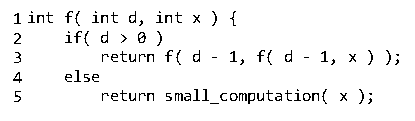
\includegraphics{just_calling_benchmark}}


The fourth microbenchmark measures the overhead of heap-allocating call frames.
This test has a very simple recursive function that calls itself twice.
At the leaves of the recursion is a very small computation, just complicated enough to prevent a smart compiler from statically computing the whole answer.
For this benchmark plain C is more than an order of magnitude faster than Charcoal.
This difference is painful, but there are several things to say about it.
First, the Charcoal implementation is a research prototype, so it is quite likely that good engineering work would close the gap to some extent.
Second, this is a microbenchmark; no application spends all of its time in calls and returns, so real application performance impact will be proportionally smaller.
Third, procedure calling in no-yield mode is just as efficient as plain C, which means that the programmer has some control over this overhead.

To investigate this foo further, ...

{\raggedleft 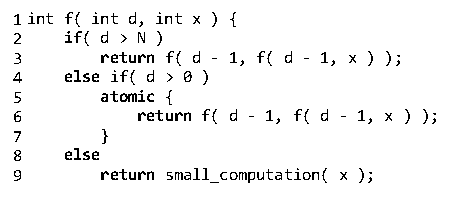
\includegraphics{just_calling_n_benchmark}}

This shows that only the N closest calls to the leaves need to be in no-yield mode for calling overhead to get below XX\%.

just calling: C: 590  Charcoal: 13

\subsection{Yielding}

The yield primitive is implemented to be very fast when the current activity will continue executing (i.e. not switch to another activity).
The key implementation trick here is described in section \ref{sec:blah}.
Even with this clever implementation, yielding is still not free.
To quantify its expense, we benchmarked a simple but problematic function: \texttt{strcmp}.
\texttt{strcmp} is tricky for a few reasons:
First, the input strings could be very long, so it is not acceptable to make the implementation simply never yield.
Second, the body of the loop is extremely simple; good implementations are just a few assembly instructions.
This means that yielding every iteration would cause significant performance overhead.
Third, whether each iteration executes depends on the computation of the previous iteration, so simple loop tiling/blocking tricks don't work.
The best-performing implementation we have found so far looks like:

{\raggedleft 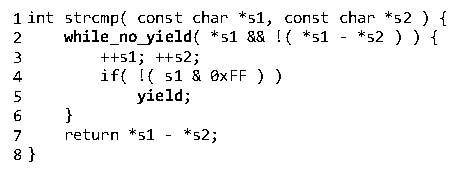
\includegraphics{strcmp_benchmark}}

\texttt{while\_no\_yield} is a special variant of the regular while loop that does not have an implicit yield after every iteration.
This is different from wrapping a regular while loop in \texttt{no\_yield}, because the latter would prevent nested yields from happening, whereas the former does not.

In the code about \texttt{B} is a bit-mask with some number of the low bits set to one.
The effect is that once every $2^N$ iterations there is a yield, where $N$ is the number of bits set in the mask.
This implementation gets the overhead down to 15\% (???), which is neither awful nor good enough to never think about this issue again.
One reasonable workaround is that when callers of \texttt{strcmp} are certain that the strings are not especially long, they can make the call in no-yield mode.
In this case, it should be just as efficient as plain C.

strcmp: C: 1000 Charcoal: 100

\subsection{Code Size}

\subsection{Microbenchmark Summary}

\section{Foreign Code}

Foreign code (including legacy code) will never yield.  This could lead
to starvation pretty easily.  Here are three strategies:

\begin{itemize}
\item Do nothing.
  Just run the foreign code.
  This is a perfectly reasonable strategy as long as the foreign code does not run for a long time.
\item Run the foreign code in its own thread.
  If it has not returned by the end of some time slice, pause it to allow other activities to run.
  This runs the risk of creating atomicity violations galore.
  It also reintroduces the possibility of data races.
  However, it might be a reasonable strategy in situations where there is very little sharing between the foreign code and the rest of the application.
\item Run the foreign code in its own thread, but only interrupt it at special ``safe-ish'' points, like system calls.
  This is a compromise between the previous two strategies in the sense that it opens the door to both starvation and atomicity violations, but provides some (imperfect) protection against both.
\end{itemize}

We have not thought at all about what the best default is or what syntactic sugar would be nice.

Another important implementation issue to consider is foreign code that calls back in to activity-aware code.
There will definitely be some fancy footwork necessary there, no matter which strategy is used.

\section{Related Work}

Continuation Passing C.

Threads without the Pain

\section{Summary and Discussion}

In this paper we introduced pseudo-preemptive threads, a new concurrency primitive, called activities for short.
Activities have advantages in reliability, composability and/or maintainability over the most common approaches to writing multitasking software (events, threads and coroutines).
From an application programmer's perspective activities feel most like threads, but they do not suffer from several of the nasty concurrency problems that plague multithreaded software.
Activities can be thought of as actually working the way inexperienced programmers think threads work.

One weakness that activities share with most multitasking frameworks is that activities cannot easily be run in parallel.
Naively running activities simultaneously on parallel processors would immediately violate the simple sequential memory model.
However, it is interesting to consider what it would take to run activities in parallel without violating their semantics.
The most obvious way to accomplish that would be with a transactional memory system; every activity would always be running in a transaction.
Yielding would cause one transaction to end and the next to begin.

The authors are not optimistic that such a transaction based system would work well, but similar things have been tried. (Stone OCM)

\cite{ONeill2015}

\acks

Acknowledgments, if needed.

% We recommend abbrvnat bibliography style.

\bibliographystyle{abbrvnat}

% The bibliography should be embedded for final submission.

\bibliography{../../../../Documents/PapersForReferencing/biy_all_research.bib}

%% \begin{thebibliography}{../../../../Documents/PapersForReferencing/biy_all_research.bib}
%% \softraggedright

%% \end{thebibliography}

\end{document}
